% Created 2017-01-21 Sat 16:21
\documentclass[presentation]{beamer}
\usepackage[utf8x]{inputenc}
\usepackage[T1]{fontenc}
\usepackage{fixltx2e}
\usepackage{graphicx}
\usepackage{longtable}
\usepackage{float}
\usepackage{wrapfig}
\usepackage{rotating}
\usepackage[normalem]{ulem}
\usepackage{amsmath}
\usepackage{textcomp}
\usepackage{marvosym}
\usepackage{wasysym}
\usepackage{amssymb}
\usepackage{hyperref}
\tolerance=1000
\usepackage{minted}
\usetheme{metropolis}
\setbeamertemplate{frame footer}{\color{lightgray}Erwin Rooijakkers, Jeroen Bruijn, Ruud Hendrikx \& Elisa Aachterberg - Blockchain and Beyond}
\metroset{block=fill}
\usetheme{default}
\author{Erwin Rooijakkers, Jeroen Bruijn, Ruud Hendrikx \& Elisa Aachterberg}
\date{21-01-2017}
\title{Blockchain and Beyond}
\hypersetup{
  pdfkeywords={},
  pdfsubject={},
  pdfcreator={Emacs 25.1.1 (Org mode 8.2.10)}}
\begin{document}

\maketitle

\begin{frame}[label=sec-0-1]{Agenda}
\begin{itemize}
\item Consensus
\begin{itemize}
\item Distributed consensus
\end{itemize}
\item Blockchain
\begin{itemize}
\item What is the blockchain?
\item Hashing, public key cryptography, P2P-networking, consensus algorithms, Merkle trees
\end{itemize}
\item \alert{Bitcoin}
\item Meditation session
\item \alert{Ethereum}
\begin{itemize}
\item White paper
\item Smart contracts
\end{itemize}
\item Blockchain applications
\item Beyond
\end{itemize}
\end{frame}

\section{Consensus}
\label{sec-1}
\begin{frame}[label=sec-1-1]{Consensus}
\begin{itemize}
\item How to \alert{confidently} and \alert{securely} transfer \alert{values} (e.g. money or digital asset)?
\item Use third-party ledger (e.g. your bank)???
\item \alert{No}, we want \alert{distributed consensus}
\item And a \alert{non-refutable}, \alert{uncompromisable} and \alert{unbreakable record} of data
\end{itemize}
\end{frame}
\section{The blockchain}
\label{sec-2}
\begin{frame}[label=sec-2-1]{What is the blockchain?}
\begin{quotation}
"A shared, programmable, cryptographically secure and therefore trusted ledger
which no single user controls and which can be inspected by everyone." -- Klaus
Schwab (Chairman World Economic Forum)
\end{quotation}
\end{frame}

\begin{frame}[label=sec-2-2]{What is the second-generation blockchain?}
\begin{quotation}
"A programming language that allows users to write more sophisticated smart
contracts [more complex applications involving having digital assets being
directly controlled by a piece of code implementing arbitrary rules, Ethereum
White Paper], thus creating invoices that pay themselves when a shipment arrives
or share certificates which automatically send their owners dividends if profits
reach a certain level." (The Economist)
\end{quotation}
\end{frame}

\begin{frame}[label=sec-2-3]{What is the blockchain?}
\begin{itemize}
\item Two kinds of \alert{records}:
\begin{itemize}
\item Transactions
\item Blocks: batches of \alert{valid transactions} that are hashed and encoded into a \alert{Merkle tree}
\end{itemize}
\item Each block includes the \alert{hash} of the \alert{prior} block in the blockchain, linking the two.
\item \alert{Decentralized} (eliminate risk of data held centrally)
\item Every \alert{node} or \alert{miner} has whole copy
\begin{itemize}
\item No \alert{centralized} "official" copy
\end{itemize}
\item Data is \alert{incorruptible}
\item \alert{Quality} by massive data \alert{replication} and \alert{computational trust}
\end{itemize}
\end{frame}
\begin{frame}[label=sec-2-4]{P2P networking}
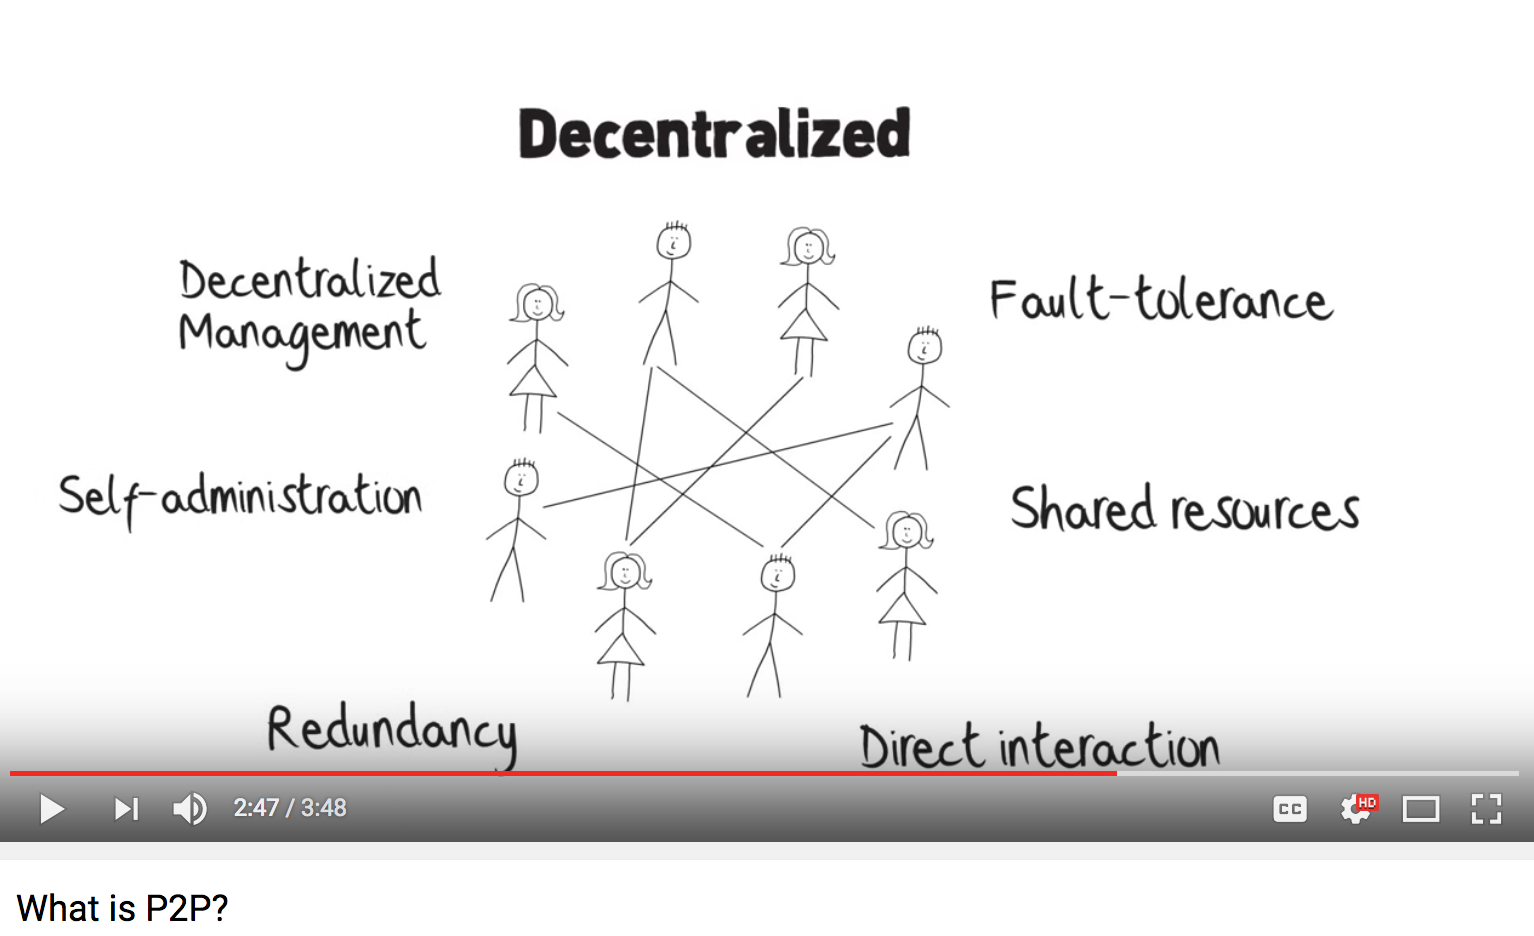
\includegraphics[width=.9\linewidth]{../images/p2p.png}
\end{frame}

\begin{frame}[label=sec-2-5]{Public key cryptography}
\begin{itemize}
\item A \alert{public key}
\begin{itemize}
\item (a long, randomly-generated string of numbers) is an address on the blockchain. Bitcoins sent across the network are recorded as belonging to that address.
\end{itemize}
\item A \alert{private key} is like a password that gives its owner access to their digital assets or otherwise interact with the various capabilities that blockchains now support.
\end{itemize}

\begin{alertblock}{Public Key Cryptography - Computerphile}
\url{https://youtu.be/GSIDS_lvRv4}


\begin{itemize}
\item A \alert{public key}
\begin{itemize}
\item (a long, randomly-generated string of numbers) is an address on the blockchain. Bitcoins sent across the network are recorded as belonging to that address.
\end{itemize}
\item A \alert{private key} is like a password that gives its owner access to their digital assets or otherwise interact with the various capabilities that blockchains now support.
\end{itemize}
\end{alertblock}

\begin{alertblock}{Public Key Cryptography - Computerphile}
\url{https://youtu.be/GSIDS_lvRv4}
\end{alertblock}
\end{frame}

\begin{frame}[label=sec-2-6]{Hashing}
\begin{itemize}
\item A \alert{hash function} is any function that can be used to map data of arbitrary size to data of fixed size
\end{itemize}
\end{frame}

\begin{frame}[label=sec-2-7]{Consensus}
\begin{itemize}
\item \alert{Proof of work}: the current difficulty in bitcoin network requires miners to try quadrillions of times before finding a nonce that fits.
\begin{itemize}
\item \alert{hashing} can provide vastly different outputs on minor changes
\end{itemize}
\item \alert{Proof of stake}: mining is done by stakeholders in the ecosystem who have the strongest incentives to be good stewards of the system. (E.g., by having large amount of currency.)
\end{itemize}
\end{frame}
\begin{frame}[label=sec-2-8]{Merkle tree}
\begin{quotation}
"Merkle trees are a fundamental part of what makes blockchains tick. Although it
is definitely theoretically possible to make a blockchain without Merkle trees,
simply by creating giant block headers that directly contain every transaction,
doing so poses large scalability challenges that arguably puts the ability to
trustlessly use blockchains out of the reach of all but the most powerful
computers in the long term. Thanks to Merkle trees, it is possible to build
Ethereum nodes that run on all computers and laptops large and small, smart
phones, and even internet of things devices." (Merkling in Ethereum)
\end{quotation}
\end{frame}

\begin{frame}[label=sec-2-9]{Merkle tree (Wikipedia)}
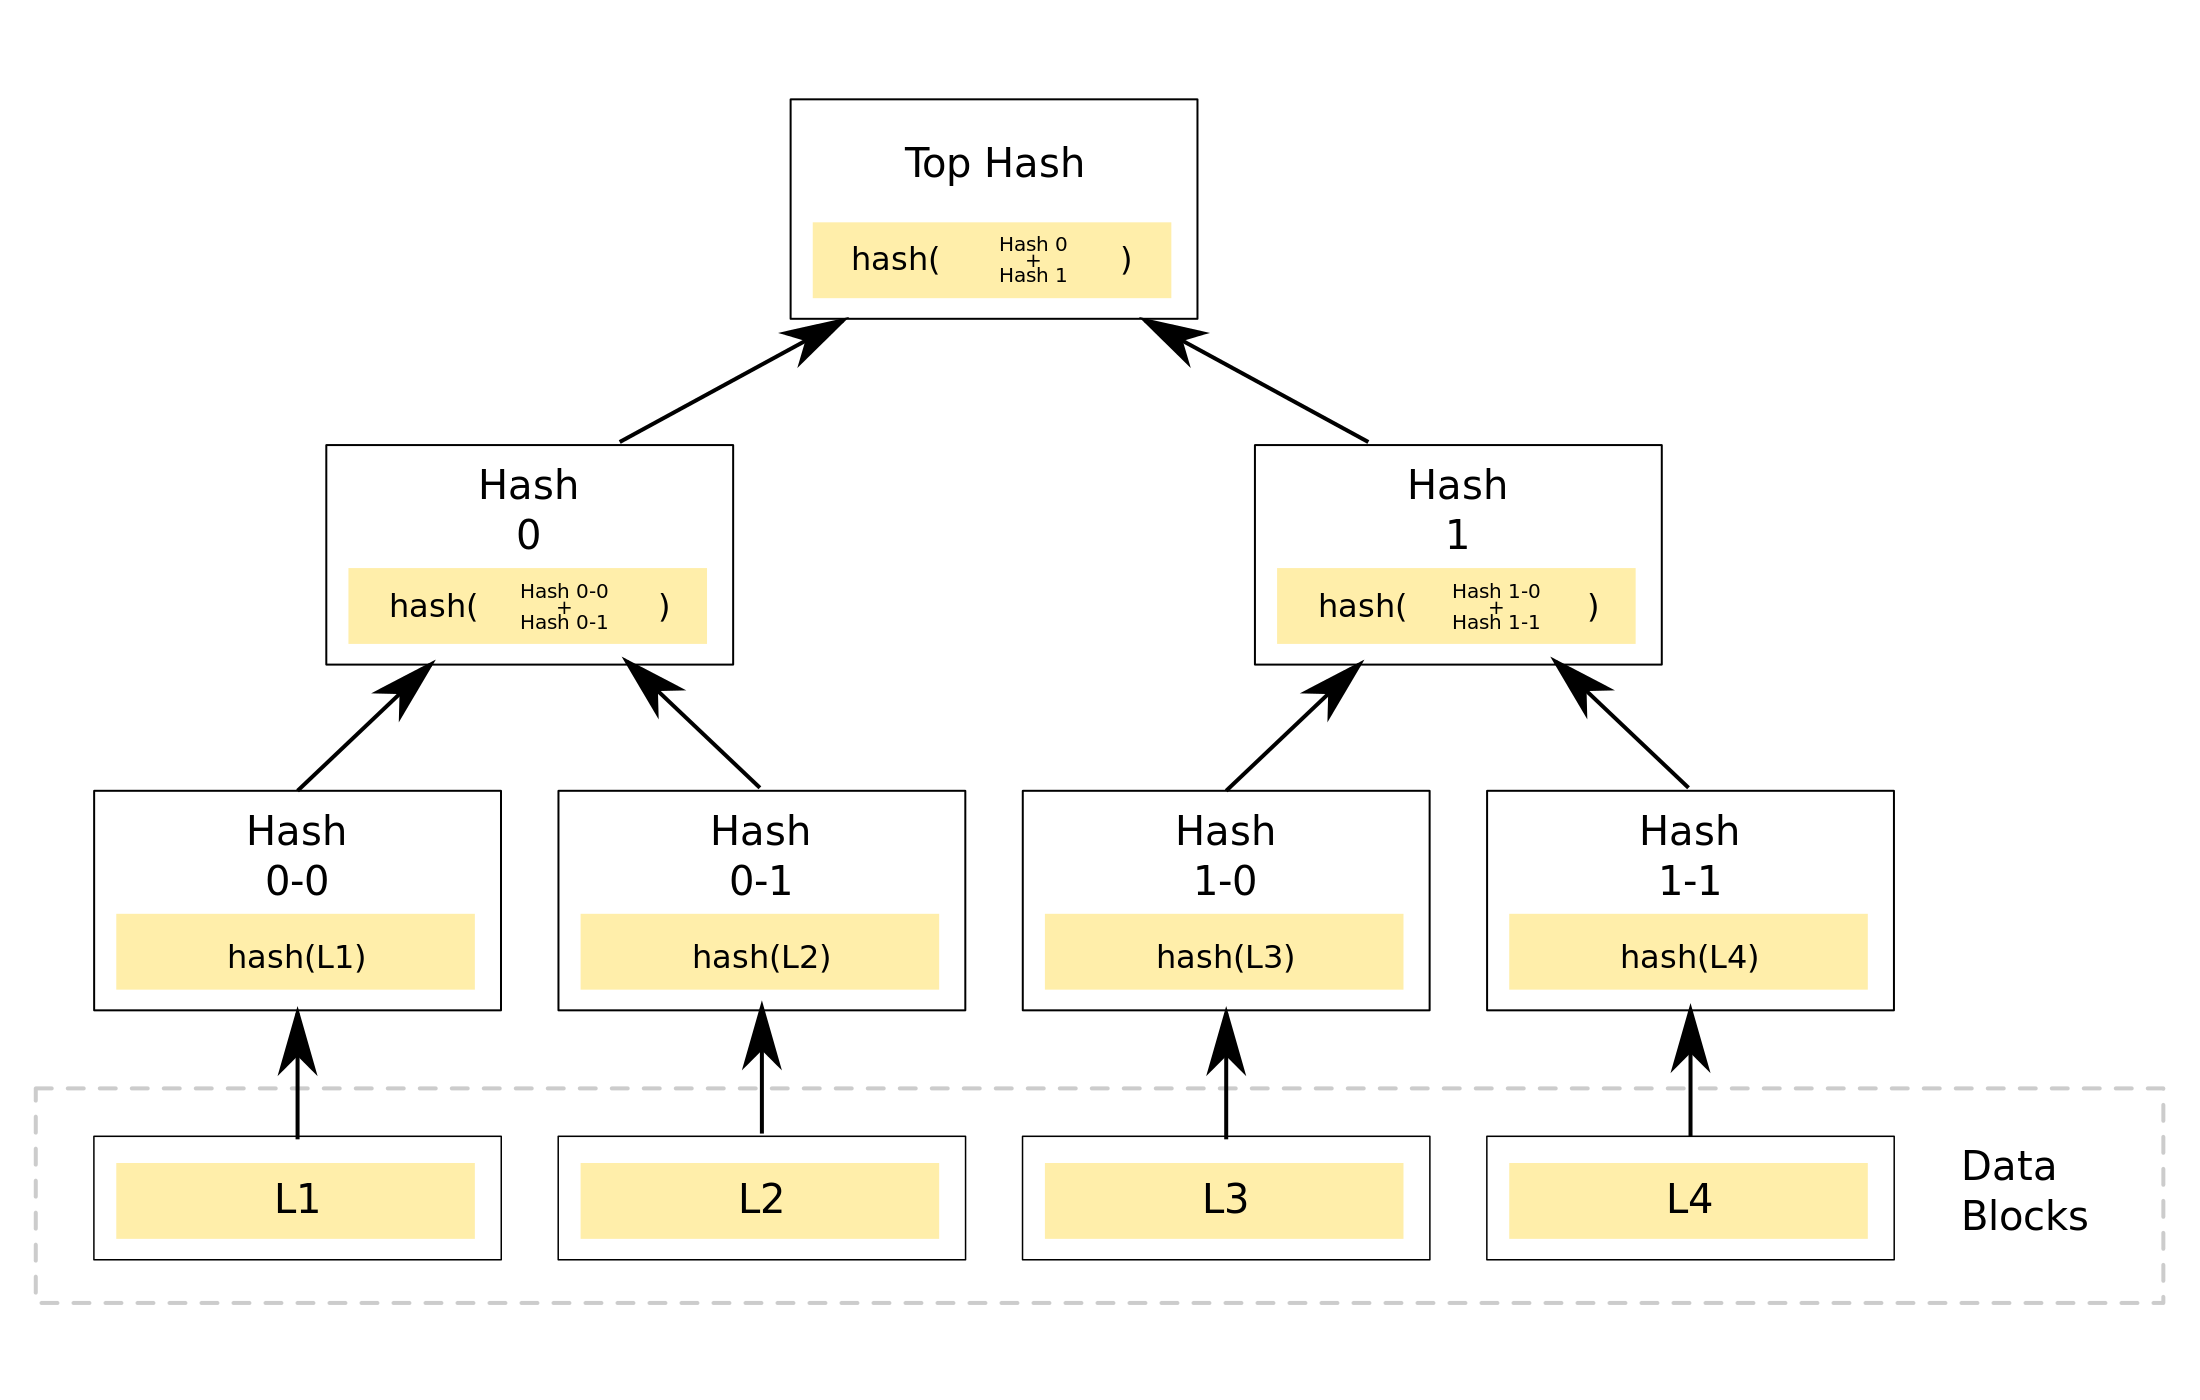
\includegraphics[width=.9\linewidth]{../images/Hash_Tree.png}
\end{frame}

\begin{frame}[label=sec-2-10]{Quiz}
\begin{itemize}
\item Demonstrating that a leaf node is a part of the given hash tree requires processing an amount of data proportional to the \alert{logarithm of the number of nodes of the tree}.
\end{itemize}
\begin{alertblock}{Quiz}
Why logarithmic?
\end{alertblock}
\end{frame}

\begin{frame}[label=sec-2-11]{Merkle proof}
\begin{itemize}
\item Someone reading the proof can verify that the hashing, at least for that branch, is consistent going all the way up the tree, and therefore that the given chunk actually is at that position in the tree.
\item If a \alert{malicious user} attempts to swap in a \alert{fake transaction} into the bottom of a Merkle tree, this change will cause a change in the node above, and then a change in the node above that, finally \alert{changing the root of the tree and therefore the hash of the block}, causing the protocol to register it as a completely different block (almost certainly with an invalid \alert{proof of work}).
\end{itemize}
\end{frame}
\begin{frame}[label=sec-2-12]{Video - ChainThat}
\begin{alertblock}{Merkle trees and hashing}
\url{https://youtu.be/lik9aaFIsl4}
\end{alertblock}
\end{frame}

\begin{frame}[label=sec-2-13]{What is a Merkle proof? (Quora)}
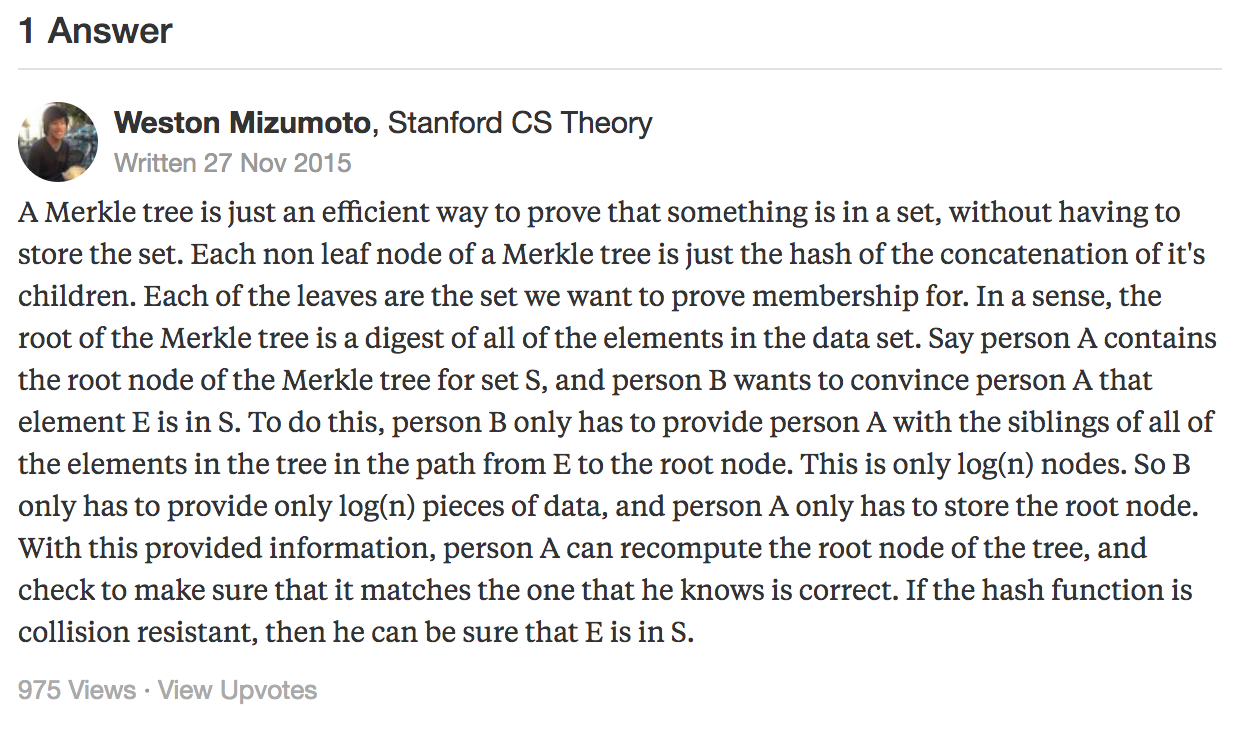
\includegraphics[width=.9\linewidth]{../images/merkle_proof.png}

\begin{alertblock}{Quiz}
What is a \alert{hash collision}?
\end{alertblock}
\end{frame}

\section{Bitcoin}
\label{sec-3}
\begin{frame}[label=sec-3-1]{What is Bitcoin?}
\begin{itemize}
\item Managing ownership
\begin{itemize}
\item through \alert{public key cryptography}
\item with \alert{consensus algorithm} for keeping track of who owns coins (known as "\alert{proof of work}")
\end{itemize}
\end{itemize}
\end{frame}

\begin{frame}[label=sec-3-2]{The first blockchain}
\begin{itemize}
\item 2008
\item The first blockchain
\item Solved the \alert{double spending problem}
\item High fault-tolerance for \alert{Byzantine Generals' Problem}
\item \alert{Public ledger}
\item Uses \alert{Merkle proofs} in order to store the transactions in every block
\item Decentralized mechanism for \alert{emergent consensus}
\begin{itemize}
\item artifact of the asynchronous interaction of thousands of independent nodes, all following simple rules.
\end{itemize}
\end{itemize}
\end{frame}
\begin{frame}[label=sec-3-3]{Video - Computerphile}
\begin{alertblock}{Bitcoin - Computerphile}
Bitcoin: \url{https://youtu.be/JyxRH18YlpA}

Problems: \url{https://youtu.be/s2XHyzPA9Zc}
\end{alertblock}
\end{frame}
\begin{frame}[label=sec-3-4]{The Bitcoin blockchain}
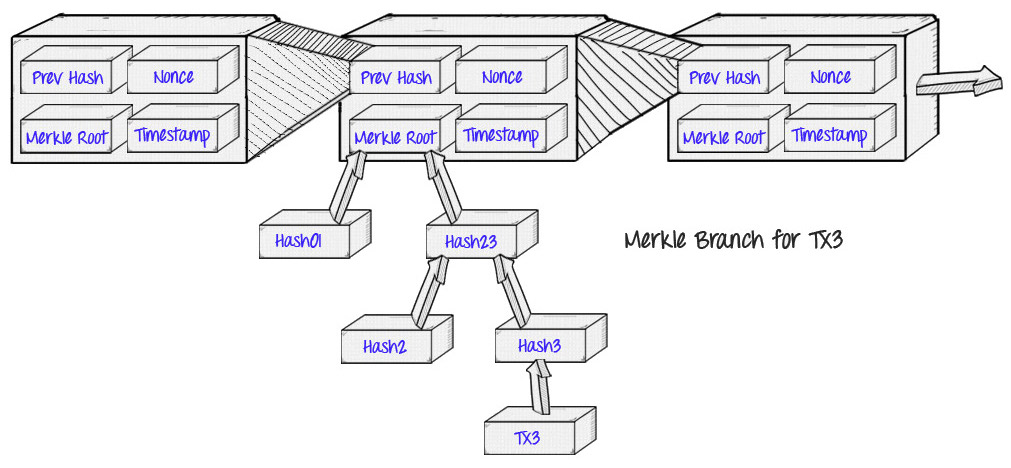
\includegraphics[width=.9\linewidth]{../images/mining.jpeg}

(\url{https://blog.ethereum.org/2015/11/15/merkling-in-ethereum/})
\end{frame}

\begin{frame}[label=sec-3-5]{The Bitcoin blockchain}
\begin{itemize}
\item Full node
\begin{itemize}
\item one that stores and processes the entirety of every block (more than one GB a month added)
\end{itemize}
\item Light node
\begin{itemize}
\item \alert{Simplified payment verification} (SPV)
\end{itemize}
\item Instead of downloading every transaction, \alert{light clients} only download the \alert{the chain of block headers}
\begin{itemize}
\item 80 bytes
\end{itemize}
\item Verification by \alert{Merkle proof}
\end{itemize}
\end{frame}
\begin{frame}[label=sec-3-6]{Problems with the Bitcoin blockchain}
\begin{itemize}
\item \alert{Follow the money}
\item Consensus Attacks
\item Blockchain forks
\begin{itemize}
\item Two candidate blocks compete to form longest blockchain
\item As both miners discover a solution for their respective candidate blocks, they immediately broadcast their own "winning" block to their immediate neighbors who begin propagating the block across the network.
\end{itemize}
\item \alert{Light clients} cannot prove anything about the currents state, like:
\begin{itemize}
\item Digital asset holdings; Name registrations; The status of financial contracts; How many bitcoins do you have right now?
\end{itemize}
\item You might need to authenticate \alert{the entire chain}!
\item Ethereum takes the concept one step further
\end{itemize}
\end{frame}

\section{Meditation session}
\label{sec-4}
\section{Ethereum}
\label{sec-5}
\begin{frame}[label=sec-5-1]{Ethereum (1)}
\begin{quotation}
"The Ethereum protocol was originally conceived as an upgraded version of a
cryptocurrency, providing advanced features such as on-blockchain escrow,
withdrawal limits, financial contracts, gambling markets and the like via a
highly generalized programming language. The Ethereum protocol would not
"support" any of the applications directly, but the existence of a
Turing-complete programming language means that arbitrary contracts can
theoretically be created for any transaction type or application."
\end{quotation}
\end{frame}

\begin{frame}[label=sec-5-2]{Ethereum (2)}
\begin{quotation}
"What is more interesting about Ethereum, however, is that the Ethereum protocol moves far
beyond just currency. Protocols around decentralized file storage, decentralized
computation and decentralized prediction markets, among dozens of other such
concepts, have the potential to substantially increase the efficiency of the
computational industry, and provide a massive boost to other peer-to-peer
protocols by adding for the first time an economic layer. Finally, there is also
a substantial array of applications that have nothing to do with money at all."
(Ethereum White Paper)
\end{quotation}
\end{frame}
\begin{frame}[label=sec-5-3]{Videos - Ethereum}
\begin{alertblock}{Ethereum the World Computer}
\url{https://youtu.be/j23HnORQXvs}
\end{alertblock}
\end{frame}

\begin{frame}[label=sec-5-4]{Three Merkle threes per block header}
\begin{itemize}
\item \alert{Transactions} tree
\item \alert{Receipts} tree
\item \alert{State} tree
\item Unlike transaction history, state can be \alert{updated}
\item Not a \alert{Merkle (binary) tree}, but a \alert{Patricia tree}
\begin{itemize}
\item New root value needs to be calculated after insertion, update, or delete.
\item \alert{Bounded depth} (against DDOS [denial of service] attacks)
\item \alert{16 children} per node
\item Root value only \alert{depends on data}, not on \alert{order}
\item \alert{path} trough the tree towards particularly value is encoded
\end{itemize}
\end{itemize}
\end{frame}

\begin{frame}[label=sec-5-5]{Facilitates things like}
\begin{itemize}
\item Has this transaction been included in a particular block? (\alert{transaction tree})
\item Tell me all instances of an event of type X (eg. a crowdfunding contract reaching its goal) emitted by this address in the past 30 days (\alert{receipt three})
\item What is the current balance of my account? (\alert{state tree})
\item Does this account exist? (\alert{state tree})
\item Pretend to run this transaction on this contract. What would the output be? (\alert{state tree, special!})
\begin{itemize}
\item \alert{Merkle state transition proof}
\end{itemize}
\end{itemize}
\end{frame}

\begin{frame}[label=sec-5-6]{Merkle state transition proof}
\begin{itemize}
\item If you run transaction \alert{T} on the state with root \alert{S}, the result will be a state with root \alert{S}, with log \alert{L} and output *O*”
\item “output” exists as a concept in Ethereum because every transaction is a function call.

\item Enables the coding of \alert{smart contracts} that will execute when specified conditions are met.
\item \alert{Extensible programming instructions} which both define and execute an agreement.
\item Ethereum is an open source blockchain project that is built specifically to realize this possibility by implementing a \alert{Turing-complete} programming language capability to implement such contracts
\end{itemize}
\end{frame}

\begin{frame}[fragile,label=sec-5-7]{Serpent}
 \begin{itemize}
\item Token System
\end{itemize}

\begin{minted}[bgcolor=white,frame=lines]{python}
def send(to, value):
    if self.storage[msg.sender] >= value:
       self.storage[msg.sender] =
	       self.storage[msg.sender] - value
       self.storage[to] =
	       self.storage[to] + value
\end{minted}
\end{frame}

\begin{frame}[fragile,label=sec-5-8]{Serpent}
 \begin{itemize}
\item A basic smart contract for a name registration system (e.g., like DNS, used in mapping domain names to IP-addresses)
\end{itemize}

\begin{minted}[bgcolor=white,frame=lines]{python}
def register(name, value):
    if !self.storage[name]:
      self.storage[name] = value
\end{minted}
\begin{itemize}
\item All it is is a \alert{database inside the Ethereum network} that can be added to, but not modified or removed from
\begin{itemize}
\item \alert{Immutability}
\end{itemize}
\end{itemize}
\end{frame}
\section{Applications}
\label{sec-6}
\begin{frame}[label=sec-6-1]{The immense potential}
\begin{quotation}
"With blockchain, we can imagine a world in which contracts are embedded in
digital code and stored in transparent, shared databases, where they are
protected from deletion, tampering, and revision. In this world every agreement,
every process, every task, and every payment would have a digital record and
signature that could be identified, validated, stored, and shared.
Intermediaries like lawyers, brokers, and bankers might no longer be necessary.
Individuals, organizations, machines, and algorithms would freely transact and
interact with one another with little friction. This is the immense potential of
blockchain." (Harvard Business Review, 2017)
\end{quotation}
\end{frame}

\begin{frame}[label=sec-6-2]{Applications currently}
\begin{itemize}
\item Cryptocurrencies
\item Georgia: blockchain based *property-*registry
\item Factom as a \alert{distributed registry}
\item Gems for \alert{decentralized messaging}
\item MaidSafe for \alert{decentralized applications}
\item Storj for a \alert{distributed cloud}
\item Tezos for \alert{decentralized voting}
\item Online \alert{voting}
\item \alert{Medical records}
\item Smart contracts (reduce moral hazards)
\item Identity management
\item \url{http://www.electricchain.org/}
\item \ldots{}
\end{itemize}
\end{frame}

\begin{frame}[label=sec-6-3]{Future}
\begin{alertblock}{Vitalik Buterin explains Ethereum}
\url{https://youtu.be/TDGq4aeevgY}
\end{alertblock}
\end{frame}
\begin{frame}[label=sec-6-4]{Sustainability}
\begin{itemize}
\item Smart energy
\item \alert{Virtual power plants} (VPPs)
\begin{itemize}
\item represent energy generating resources that are connected across a smart grid but \alert{that aren’t necessarily concentrated in one central location}, such as traditional power plants
\end{itemize}
\end{itemize}
\end{frame}
\begin{frame}[label=sec-6-5]{Sustainability}
\begin{quotation}
"Distributed energy is really about generating your own energy, being self-reliant, selling excess energy to others."
\end{quotation}

\begin{quotation}
"Distributed energy is really about generating your own energy, being self-reliant, selling excess energy to others."
"Blockchain is not only useful in moving money, it’s useful in moving any asset in a very transparent and reliable way,"
\end{quotation}
\end{frame}
\begin{frame}[label=sec-6-6]{Problems with Ethereum}
\begin{itemize}
\item \alert{Scalability}
\item \alert{Centralization} risk (because of growth of blockchain only few organisations with full node)
\end{itemize}
\end{frame}

\section{Demo}
\label{sec-7}
\begin{frame}[label=sec-7-1]{Sources}
\begin{itemize}
\item \url{https://en.wikipedia.org/wiki/Blockchain_(database)}
\item \url{https://blog.ethereum.org/2015/11/15/merkling-in-ethereum/}
\item \url{https://monax.io/explainers/permissioned_blockchains/}
\item \url{https://www.linkedin.com/pulse/consensus-mechanisms-used-blockchain-ronald-chan}
\item \url{https://github.com/ethereum/wiki/wiki/White-Paper}
\end{itemize}
\end{frame}

\begin{frame}[label=sec-7-2]{To watch}
\begin{itemize}
\item \url{http://www.ted.com/talks/don_tapscott_how_the_blockchain_is_changing_money_and_business}
\item \url{https://www.youtube.com/channel/UC6rYoXJ_3BbPyWx_GQDDRRQ}
\end{itemize}
\end{frame}
% Emacs 25.1.1 (Org mode 8.2.10)
\end{document}
